Stadia can be classified as an augmented service as the main purchasable is a subscription-based service that can't be access without a sufficiently high internet speed connection (a minimum of 10Mbps according to their website \cite{stadiaSupport}) so it can't 
be a product as a product must be tangible and can be consumed at will without a special requirement(internet connection).

\begin{figure}[H]
    \centering
    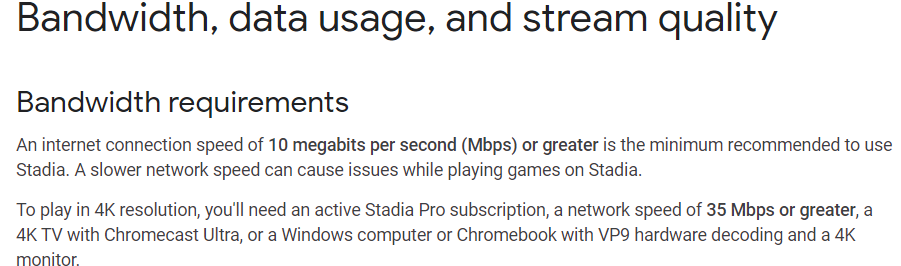
\includegraphics[width=13cm]{images/bandwidth.png}
    \caption{Screen Capture Of Internet Requirement}
    \label{fig:internetReq}
\end{figure}

As for the augmented part, Stadia subscriptions include (optional) products to use 
with the service such as the stadia controller.

\begin{figure}[H]
    \centering
    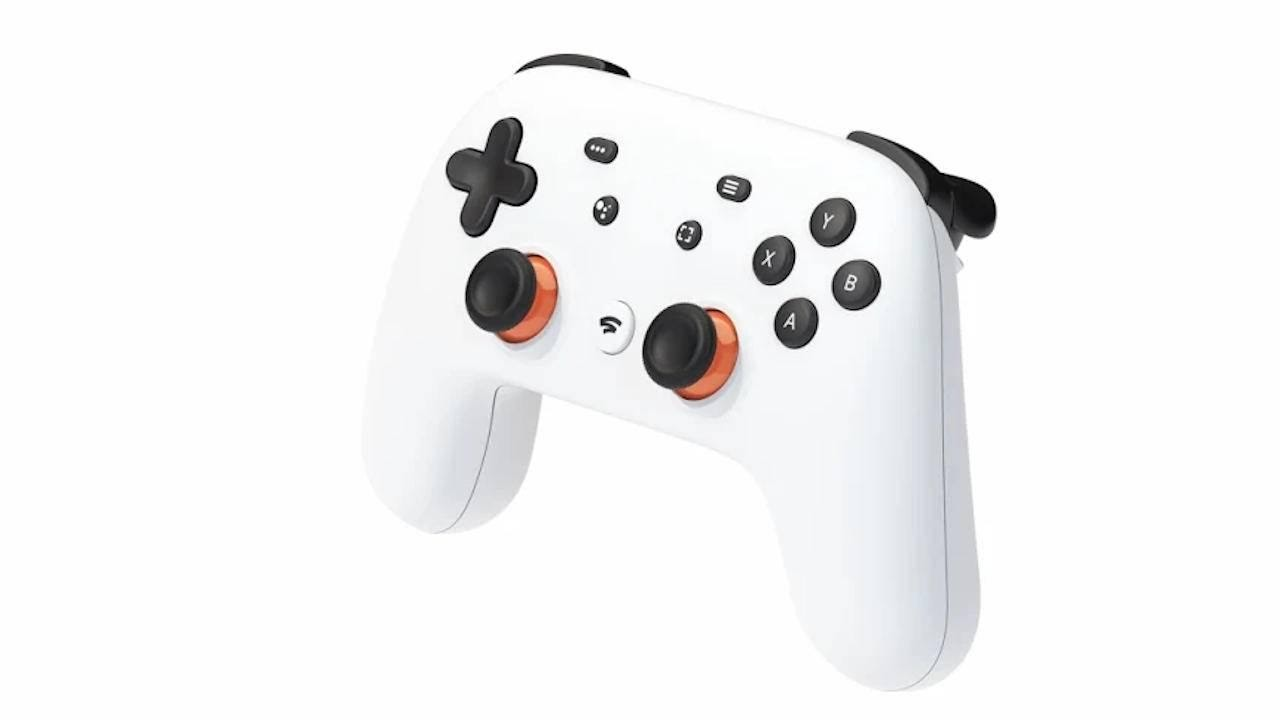
\includegraphics[width=10cm]{images/controller.jpg}
    \caption{Google Stadia Controller}
    \label{fig:controller}
\end{figure}

In conclusion, google stadia is a service with optional products to enhance the 
experience.
